\chapter{Implementation}
\label{sec:implementation}

\section{Implementation Overview}
AutoReturn was implemented as a native \textbf{PySide6} desktop application with a modular backend centered on an \textbf{Orchestrator} class \cite{pyside2024}. The implementation combines platform-specific agents, configurable automation services, and model-assisted processing for summarization, drafting, extraction, and tone-aware assistance. Gmail and Slack connectivity rely on the official platform APIs \cite{gmail2023,slack2023}, while account ownership and authentication are coordinated through a Supabase-backed identity layer \cite{supabase2024}. The final codebase prioritizes controllable automation over fully autonomous behavior, so high-risk actions are still guarded by explicit policy checks, confidence rules, or user review steps.

This chapter focuses on the final implemented state of the system rather than on intermediate concepts from earlier project phases. It therefore summarizes the completed modules, the main engineering challenges, the recurring implementation patterns, and the interface views that best represent the final prototype.

\section{Module Details}
This section summarizes the final implemented modules so that the report can connect design claims with concrete development outcomes. The following tables provide a compact view of the completed functionality present in the final AutoReturn prototype.

\begin{table}[!htbp]
\centering
\caption{AutoReturn Module Details -- Part I}
\label{tab:implementation}
\footnotesize
\renewcommand{\arraystretch}{1.15}
\setlength{\tabcolsep}{5pt}
\begin{adjustbox}{width=\textwidth}
\begin{tabular}{|>{\raggedright\arraybackslash}p{4.8cm}|>{\raggedright\arraybackslash}p{8.7cm}|}
\hline
\textbf{Module} & \textbf{Implementation Details} \\
\hline
Priority of email/message & Weighted urgency assessment combines keyword, deadline, and sender signals through the priority engine. \\
\hline
Email/message summary & AI-assisted summaries are generated for synchronized Gmail and Slack messages through the model-backed service layer. \\
\hline
Draft generation & Draft generation is integrated into the unified workflow and supports downstream review, tone adjustment, and policy checks. \\
\hline
Plain text response & Plain-reply review dialogs and policy-aware sending are implemented for controlled response workflows. \\
\hline
Task classification & Model-assisted task and intent classification is integrated into the automation workflow for actionable message understanding. \\
\hline
Task extraction & Structured task and event extraction are supported for messages that contain actionable or schedulable content. \\
\hline
Unified inbox & Gmail and Slack content is normalized into a shared message flow for display and downstream processing. \\
\hline
Orchestrator & A central orchestrator coordinates routing, shared services, and platform-specific agent interaction. \\
\hline
Gmail agent & Message retrieval, reading, summarization, drafting, and automation support are integrated through the Gmail agent. \\
\hline
Slack agent & Slack message retrieval, unified-inbox integration, and downstream workflow support are implemented through the Slack agent. \\
\hline
Tone preference & Tone recommendation and draft adjustment are handled through the tone engine with configurable preferences and conservative fallbacks. \\
\hline
Event-driven file lookup & The attachment resolver searches approved paths, blocks ambiguous auto-attachment, and requests manual confirmation when needed. \\
\hline
Search & Search is supported across the desktop workflow and is also integrated into voice-triggered UI actions. \\
\hline
\end{tabular}
\end{adjustbox}
\end{table}

\begin{table}[!htbp]
\centering
\caption{AutoReturn Module Details -- Part II}
\footnotesize
\renewcommand{\arraystretch}{1.15}
\setlength{\tabcolsep}{5pt}
\begin{adjustbox}{width=\textwidth}
\begin{tabular}{|>{\raggedright\arraybackslash}p{4.8cm}|>{\raggedright\arraybackslash}p{8.7cm}|}
\hline
\textbf{Module} & \textbf{Implementation Details} \\
\hline
Desktop and pop-up notifications & Notification dialogs, unread tracking, and controlled desktop-alert behavior are implemented in the desktop client. \\
\hline
Website and deployment & A public project website is available and deployed for presentation and external project overview purposes. \\
\hline
.deb package & Packaging support is included as part of the deliverable direction for installation and distribution of the desktop application. \\
\hline
Sender statistics & Sender and tone-related usage statistics are available through the settings and tone-profile interfaces. \\
\hline
Calendar feature & Event extraction, conflict checks, Google Calendar insertion, and ICS export are implemented for scheduling workflows. \\
\hline
CI/CD pipeline & Structured validation and project-delivery workflow support are included as part of the final implementation and deployment process. \\
\hline
Auto reply & Auto-reply mode is implemented through the automation policy engine and remains gated by DND and policy checks. \\
\hline
DND & Do Not Disturb rules suppress or redirect response and notification behavior according to user policy settings. \\
\hline
Voice-enabled actions & Voice support includes transcription, hotkey activation, wake-mode support, and controlled UI actions within the desktop workflow. \\
\hline
Wake-word activation & Wake-word mode is supported through the integrated ``Hey AutoReturn'' activation phrase for hands-free triggering. \\
\hline
\end{tabular}
\end{adjustbox}
\end{table}

\section{Selected Technical Challenges and Solutions}
The implementation process required repeated refinement in response to ambiguity, cross-platform mismatch, and automation safety concerns. Table~\ref{tab:technical_challenges} summarizes the most important engineering challenges encountered during development and the responses adopted in the final system.

\begin{table}[!htbp]
\centering
\footnotesize
\renewcommand{\arraystretch}{1.15}
\setlength{\tabcolsep}{5pt}
\begin{adjustbox}{width=\textwidth}
\begin{tabular}{|>{\raggedright\arraybackslash}p{0.8cm}|>{\raggedright\arraybackslash}p{3.2cm}|>{\raggedright\arraybackslash}p{5.1cm}|>{\raggedright\arraybackslash}p{6.1cm}|}
\hline
\textbf{No.} & \textbf{Challenge} & \textbf{Issue} & \textbf{Implemented Response} \\ \hline
1 & Platform authentication & Gmail and Slack integration required reliable token handling and account state management. & OAuth refresh logic, account linking, and controlled authentication services were added so connected platforms could be reused safely across sessions. \\ \hline
2 & Priority ambiguity & Simple keyword matches produced weak urgency judgments, especially in negated phrases such as ``not urgent.'' & A weighted priority engine was introduced to combine keyword, deadline, and sender signals rather than relying on isolated words. \\ \hline
3 & Long-message context loss & Important requests were sometimes diluted inside long threads or mixed conversation history. & Message-cleaning and context-selection steps were added before summarization, drafting, and extraction workflows. \\ \hline
4 & Cross-platform data mismatch & Gmail and Slack expose different message structures, metadata, and identifiers. & The orchestrator normalizes content into a shared message flow so downstream services can operate consistently across both integrations. \\ \hline
5 & UI and worker concurrency & Background workers, API requests, and interface updates could interfere with one another. & Threaded execution and signal-based update paths were used to isolate slower tasks from the main interface. \\ \hline
6 & Tone-detection variability & Real-world language did not fit a purely rule-based formal/informal split. & The tone engine uses configurable rules and weighted signals, with conservative fallbacks when certainty is low. \\ \hline
7 & Attachment ambiguity & File requests could produce either no match or several plausible matches. & The attachment resolver blocks automatic completion when confidence is weak and requests manual confirmation instead. \\ \hline
8 & Reply policy safety & Automation should not treat every sender or message type equally. & Reply-policy services enforce DND, allowlists, and review-first modes before message transmission is allowed. \\ \hline
\end{tabular}
\end{adjustbox}
\caption{Selected Technical Challenges and Solutions}
\label{tab:technical_challenges}
\end{table}

\section{Implementation Patterns}
The implementation patterns in this section describe the recurring ways in which AutoReturn coordinates agents, routing logic, and assisted interaction. These patterns are important because they explain how the completed features operate together as one workflow-oriented desktop system.

\subsection{Orchestrator-Agent Coordination}
The backend is organized around an \textbf{Orchestrator} that routes work to platform-specific agents and shared services. In the current implementation, Gmail and Slack are the two primary agents, while drafting, tone recommendation, and automation settings are managed through dedicated backend components. This structure kept platform-specific logic separate from shared workflow logic and made it easier to evolve the system without rewriting the full request pipeline.

Event-related workflows also follow a standardized export path: when the system confirms a time-related item, it can prepare an ICS artifact aligned with the iCalendar interchange format \cite{rfc5545}.

\subsection{Priority Scoring}
The priority engine uses a weighted score rather than a single hard-coded rule. In simplified form, the implemented pattern can be described as:
\[
\text{urgency} = (w_k \times \text{keyword}) + (w_d \times \text{deadline}) + (w_s \times \text{sender})
\]
This design made the classifier more robust than simple keyword spotting because sender context and deadline cues can raise or lower the final urgency level.

The importance of this pattern lies in its balance between simplicity and usefulness. It provides an interpretable scoring approach that is easier to reason about than a fully opaque classifier, while still being richer than isolated keyword matching.

\subsection{Voice Command Handling}
Voice functionality is implemented as a supporting subsystem rather than the primary interaction model. The current codebase provides push-to-talk capture, transcription, wake-command parsing, and routing of recognized commands into controlled UI actions or orchestrator requests. Speech recognition in the project follows the practical desktop pattern enabled by Whisper-based tooling for local transcription workflows \cite{whisper2023}. This is useful for assisted interaction, but it is intentionally narrower than a fully conversational voice assistant.

This limited but structured role is consistent with the overall project philosophy of controlled assistance. Voice is included where it can support productivity, but it is not allowed to undermine reliability or clarity in the main communication workflows.

\section{Representative Code Snippets}
The following excerpts are intentionally brief and are included only to illustrate recurring implementation ideas from the final repository. They do not attempt to reproduce large portions of the source code, but instead show how key architectural patterns are expressed in practice.

\subsection{Base Agent Interface}
The actual backend agents share a small common contract. The report includes a shortened version of the implemented base class to illustrate this pattern:
\begin{verbatim}
class BaseAgent(ABC):
    def __init__(self, name: str):
        self.name = name

    @abstractmethod
    async def process_request(self, request):
        pass
\end{verbatim}

\subsection{Priority Engine Pattern}
The implemented priority engine follows the weighted three-signal structure shown below:
\begin{verbatim}
urgency = (w_keyword * k_score) + \
          (w_deadline * d_score) + \
          (w_sender * s_score)
\end{verbatim}
This compact pattern is more faithful to the final repository than the longer earlier pseudocode and better reflects how urgency labels are derived in practice.

Including this compact excerpt is useful because it shows that the implementation logic is not only described narratively in the report, but also reflected directly in the code structure. It therefore links the design explanation with the actual computational pattern used in the prototype.

\section{User Interface Screens}
The following figures present the principal user-interface screens of the AutoReturn desktop application. Together, they illustrate account connection, unified inbox navigation, assisted reply handling, automation settings, event workflows, and voice-related interaction points in the implemented system.

\begin{figure}[htbp]
    \centering
    \begin{subfigure}[t]{0.48\textwidth}
        \centering
        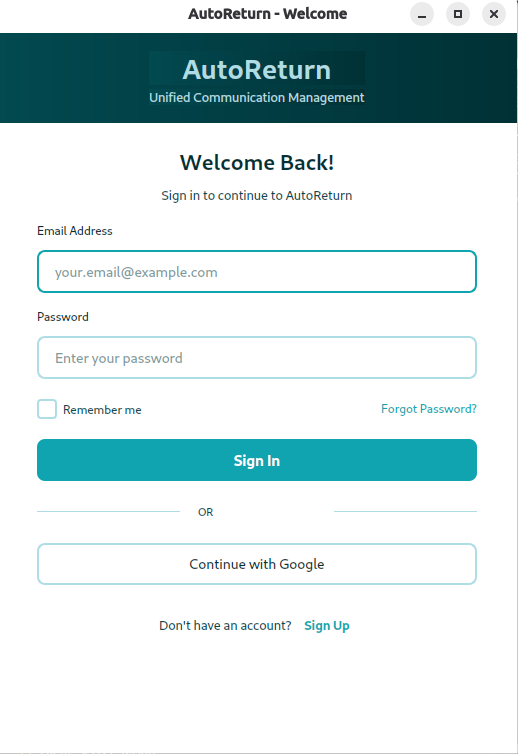
\includegraphics[width=0.70\linewidth,height=5.0cm,keepaspectratio]{Figures/Login_and_Account_Connection.png}
        \caption{Login and Account Connection}
        \label{fig:ui_login_connection}
    \end{subfigure}
    \hfill
    \begin{subfigure}[t]{0.48\textwidth}
        \centering
        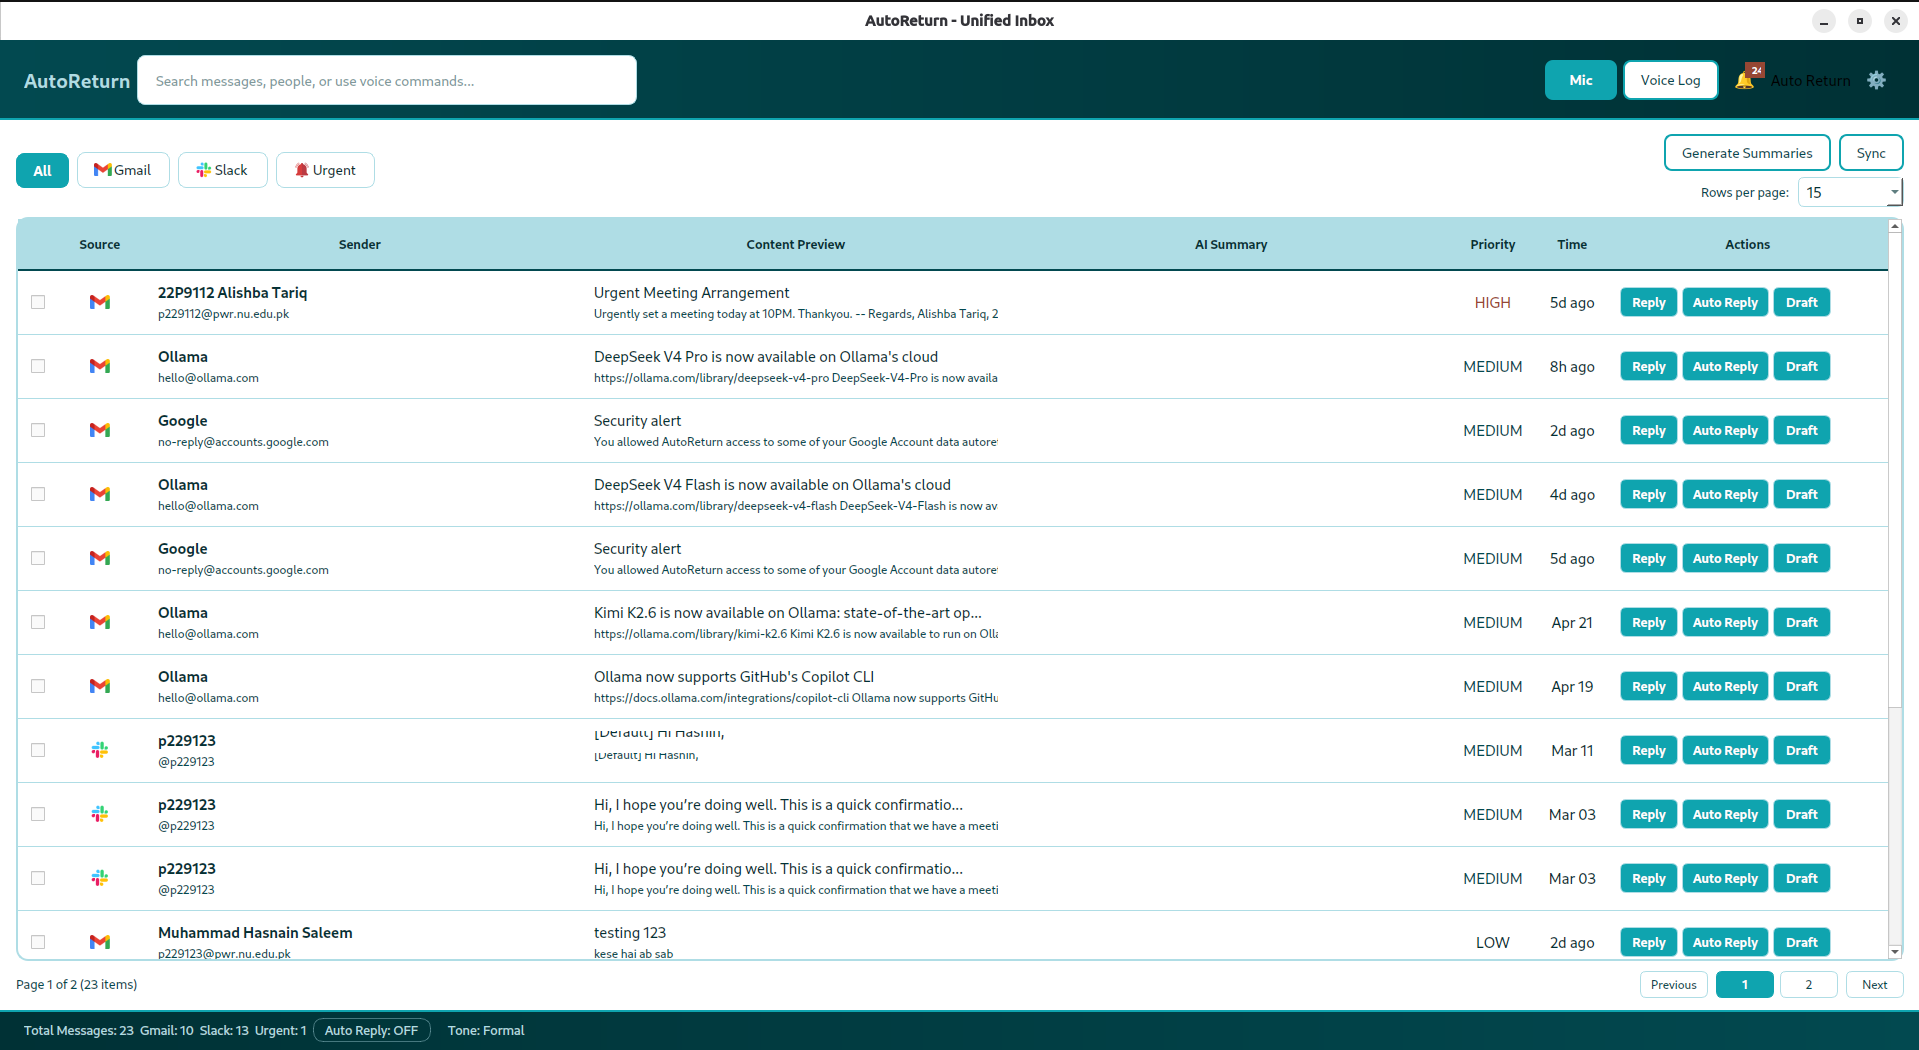
\includegraphics[width=0.98\linewidth,height=5.0cm,keepaspectratio]{Figures/Unified_Inbox_Dashboard.png}
        \caption{Unified Inbox Dashboard}
        \label{fig:ui_unified_inbox}
    \end{subfigure}

    \vspace{0.35em}

    \begin{subfigure}[t]{0.48\textwidth}
        \centering
        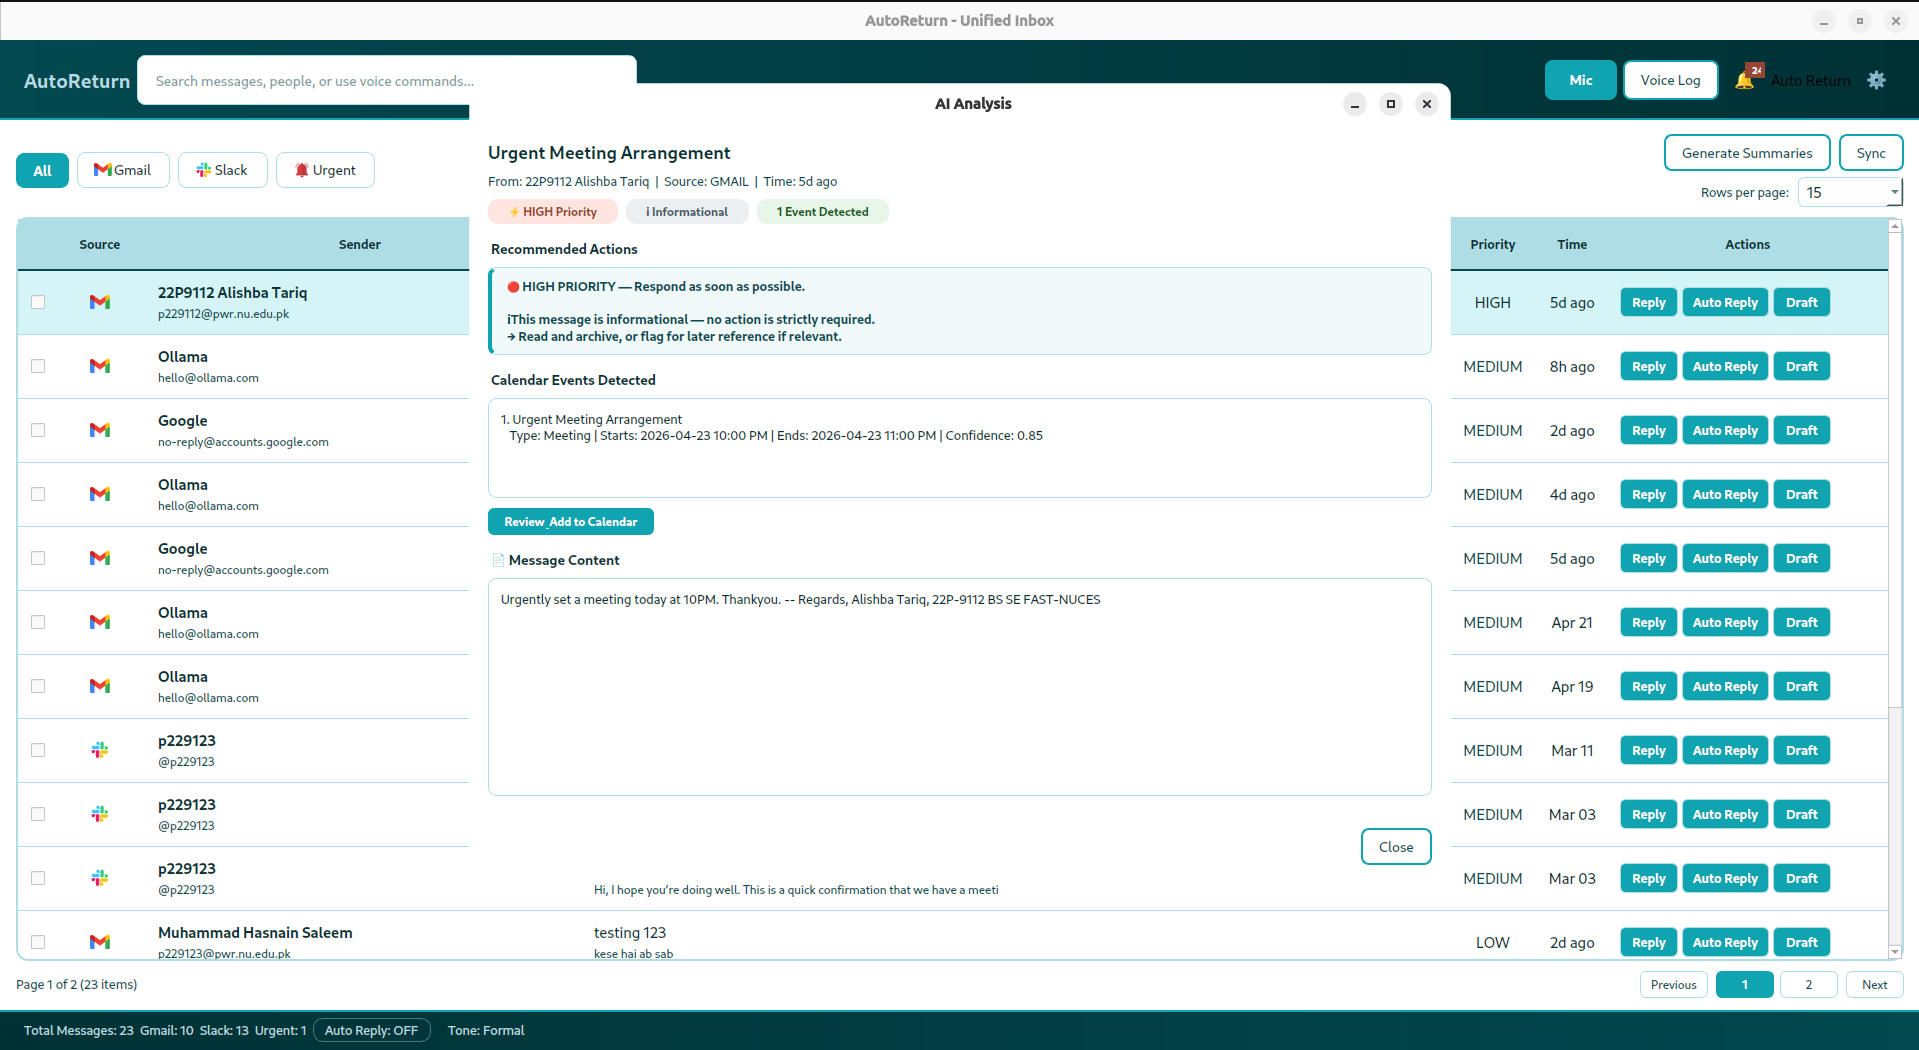
\includegraphics[width=0.98\linewidth,height=5.0cm,keepaspectratio]{Figures/Reply_Assistance.png}
        \caption{Reply Assistance}
        \label{fig:ui_reply_assistance}
    \end{subfigure}
    \hfill
    \begin{subfigure}[t]{0.48\textwidth}
        \centering
        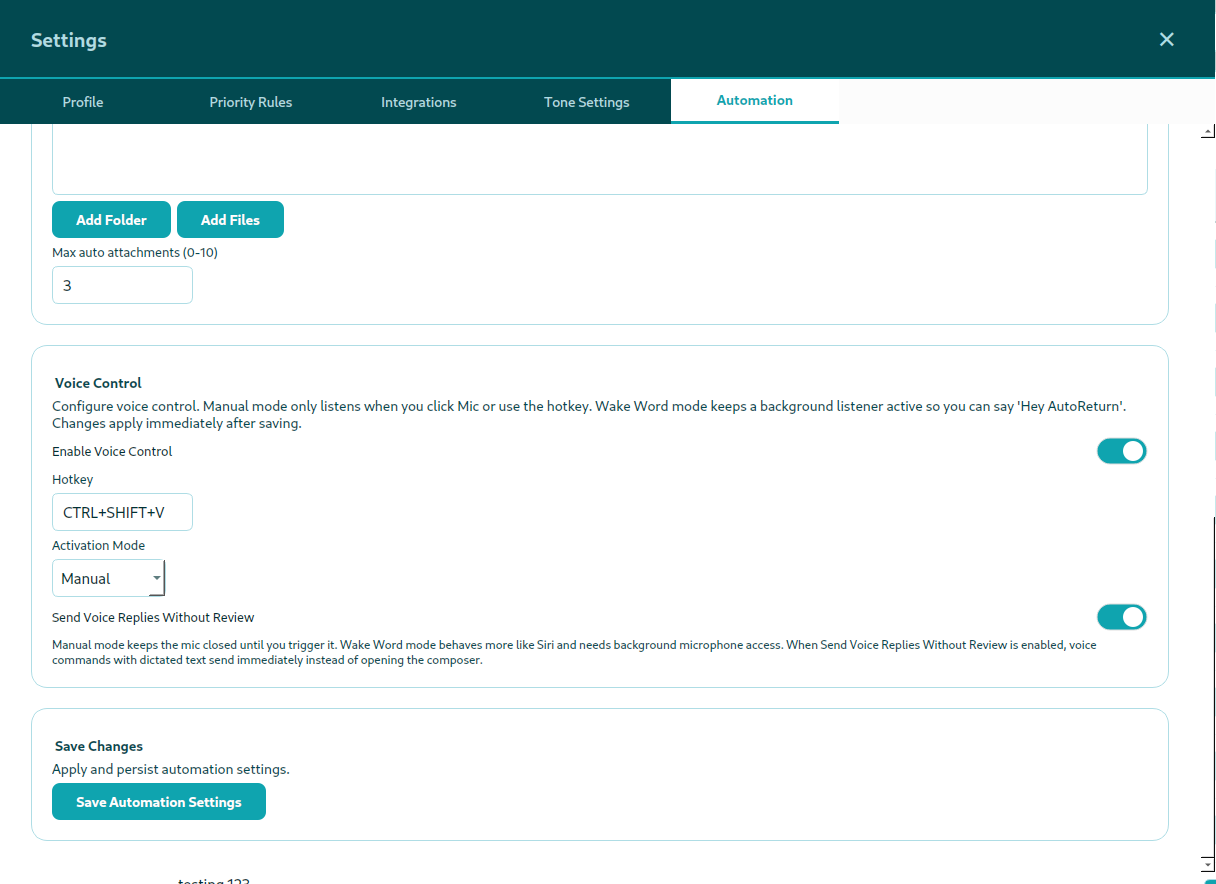
\includegraphics[width=0.98\linewidth,height=5.0cm,keepaspectratio]{Figures/Policy_Settings.png}
        \caption{Policy Settings}
        \label{fig:ui_policy_settings}
    \end{subfigure}
\caption{Primary AutoReturn Interface Screens}
\end{figure}

\begin{figure}[htbp]
    \centering
    \begin{subfigure}[t]{0.48\textwidth}
        \centering
        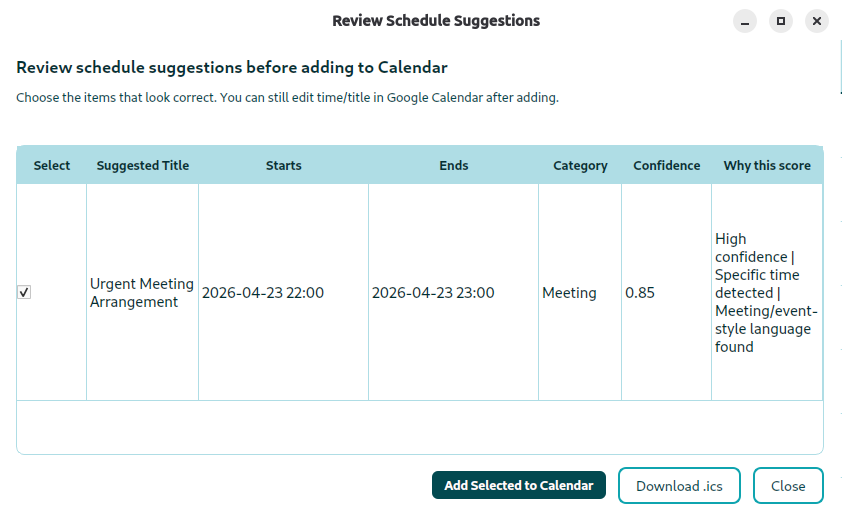
\includegraphics[width=0.98\linewidth,height=5.0cm,keepaspectratio]{Figures/Event_and_Calendar_Workflow.png}
        \caption{Event and Calendar Workflow}
        \label{fig:ui_event_workflow}
    \end{subfigure}
    \hfill
    \begin{subfigure}[t]{0.48\textwidth}
        \centering
        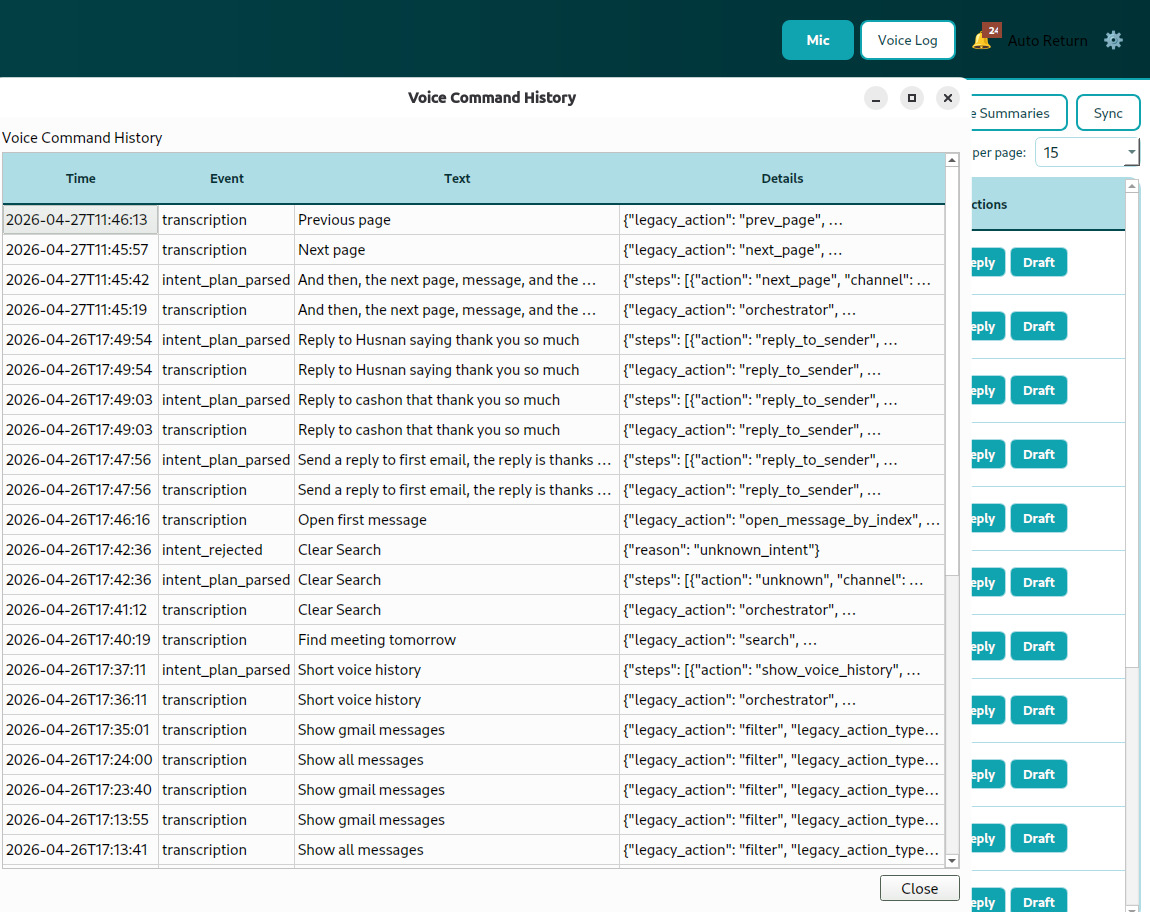
\includegraphics[width=0.98\linewidth,height=5.0cm,keepaspectratio]{Figures/Voice_Logs.png}
        \caption{Voice or Status Panel}
        \label{fig:ui_voice_status}
    \end{subfigure}
\caption{Additional AutoReturn Interface Screens}
\end{figure}

\section{Conclusion}
The final implementation demonstrates a working multi-service desktop prototype rather than an isolated proof of concept. Its strongest areas are platform integration, unified message handling, drafting support, priority assessment, and policy-aware automation. Features such as voice interaction and broader AI behavior are present but still less mature, so they are best understood as meaningful extensions of the core system rather than the primary basis of the project.

From an implementation perspective, the project shows that a modular orchestrator-agent design can support a realistic communication assistant without collapsing everything into a single opaque service layer. This provides a practical base for later refinement, broader testing, and more complete deployment support.
